\chapter{Related Work}
\label{ch:background}

This chapter reviews the literature relevant to age-conditioned behaviour in
large language models. Section~\ref{sec:primer} introduces model safeguards and
their limitations, Section~\ref{sec:children_ai} considers child-specific risks
and age assurance, and Section~\ref{sec:related_work} reviews prior empirical
work before Section~\ref{sec:gap} identifies the research gap.


% ============================================================
\section{Language Models and Safeguards}
\label{sec:primer}

Model safety depends on both post-training alignment and external safeguards.
The distinction matters here because a model refusal and a provider block are
different observable behaviours.


% ------------------------------------------------------------
\subsection{Generation and Alignment}
\label{sec:primer-foundations}

Large language models generate text autoregressively,

\begin{equation}
    p_{\theta}(x)
    =
    \prod_{t=1}^{n}
    p_{\theta}\!\left(x_t \mid x_{<t}\right),
    \label{eq:autoregressive}
\end{equation}

so information introduced earlier in the context, including a user's age,
remains available during subsequent generation. Whether the model uses that
information consistently is an empirical question rather than an architectural
guarantee.

Safety behaviour is introduced during post-training, commonly through
instruction tuning and preference optimisation. Refusal is therefore learned
rather than imposed as a deterministic rule, and may generalise unevenly beyond
the distributions represented during alignment
\cite{britoSafetyNotUniversal2026}. Safety also depends on the training procedure:
reasoning capability and alignment method can affect safety performance, while
adversarial pressure can weaken otherwise protective behaviour
\cite{liWhatMattersSafety2026,zhouHiddenRisksLarge2025}.


% ------------------------------------------------------------
\subsection{Guardrails}
\label{sec:primer-guardrails}

Guardrails inspect a model's input, output, or both and may allow, block or
modify an exchange
\cite{dongBuildingGuardrailsLarge2024,dongSafeguardingLargeLanguage2024}.
They operate outside the model's learned response policy, so a blocked exchange
must be distinguished from a refusal generated by the model itself. This
distinction is retained throughout the evaluation.

Guardrails are commonly defined through content-risk taxonomies
\cite{padhiGraniteGuardianComprehensive2025,
dongSafeguardingLargeLanguage2024}. Such taxonomies usually describe what is
requested rather than who is asking. They therefore represent age-independent
harm more naturally than cases where the same request may warrant different
responses for a child and an adult.


% ------------------------------------------------------------
\subsection{Safety Limitations}
\label{sec:primer-limitations}

Neither alignment nor guardrails guarantee stable safety. Jailbreak strategies
including role play and prompt injection can weaken refusal behaviour
\cite{liWhatMattersSafety2026}, while protection can vary across populations.
Brito et al.\ report defence-rate differences of up to 42 percentage points
within a model across demographic groups
\cite{britoSafetyNotUniversal2026}. Aggregate safety rates may therefore conceal
substantial variation between users.

Safeguards can also reduce utility by refusing legitimate requests
\cite{dongBuildingGuardrailsLarge2024,dongSafeguardingLargeLanguage2024}.
Over-restriction is particularly relevant for younger users because legitimate
questions about health, relationships or personal safety may overlap with
sensitive-content categories.

Existing safeguards are therefore imperfect, externally mediated and primarily
content-conditioned. Whether model behaviour also changes appropriately with
the age of the user remains an open empirical question.

\section{Children \& AI}
\label{sec:children_ai}

\subsection{Developmental Risks}
\label{sec:child_users}
\label{sec:risk_mechanisms}

Children and adolescents differ from adults in cognitive development, critical
literacy and privacy awareness, and chatbot interaction is conversational and
personalised, so a reply suitable for an adult may be developmentally
inappropriate for a younger user through excessive detail, validated assumptions
or complex language.

Ofcom's 2026 summary reports that AI tools are a routine part of children's media
environments \cite{ChildrensMediaLives2026}. In a
study of 17 children aged 8 to 17, participants used ChatGPT, Gemini, Copilot and
Snapchat's My AI for homework, search, image generation and entertainment
\cite{ChildrensMediaLives2026}. Minors reach general-purpose assistants despite
stated age restrictions: a nine-year-old uses ChatGPT for gaming advice and holds
a Roblox account registered as 16 to 17 after a peer used AI to bypass age
verification. The report emphasises that
safety should be assessed on the generated response, since children switch
between tools without regard to reliability or safety settings.

Kurian describes an \emph{empathy gap} in which a model mimics fluency and
attentiveness without understanding the user's developmental stage
\cite{kurianNoAlexaNo2025}. Adolescents, seeking autonomy and fuller
explanations, still need safeguards against self-harm, sexual content, eating
disorders and substance use, and treating everyone under 18 as one group
overlooks the difference between middle childhood and adolescence
\cite{TeenSafetyFreedom2026, IntroducingTeenSafety2026}.

Five mechanisms carry the risk, each implying a behaviour that can be audited.
\emph{Anthropomorphism}: a caring model can appear more socially aware than it
is, raising the risk of dependency, particularly on companion platforms where
chatbots are treated as friends \cite{kurianNoAlexaNo2025,
groganAIWillAlways2025, namvarpourUnderstandingTeenOverreliance2026}.
\emph{Personal disclosure}: children reveal age, school grade, location or family
conflict, and Figueira et al.\ argue that a conversation is itself an age-gating
setting because the interaction discloses age-related detail
\cite{figueiraActionsSpeakLouder2026}. \emph{Sycophancy}: models adapt to and
affirm user views in relational settings, and the wider literature shows
preference-optimised models favouring agreement over accuracy
\cite{groganAIWillAlways2025, garciaCharacterAI2026,
sharmaUnderstandingSycophancyLanguage2025, shahSycophancyMultilingualAlignment2026,
lambertReinforcementLearningHuman2026}. \emph{Unsafe advice}: risk varies by topic
and by level of detail, so a general discussion of a hazard and a set of
instructions for it are different objects. \emph{Multi-turn drift}: providers
acknowledge that safeguards weaken in long interactions on sensitive topics
\cite{HelpingPeopleWhen2026, HelpingChatGPTBetter2026}, which is why evaluation
here runs across turns.

\subsection{Age Signals and Assurance}
\label{sec:definitions}
\label{sec:age_assurance}

A child's input differs from an adult's in two ways. An \emph{age signal} is
information in the input that reveals the user's age, taking two forms
(Figure~\ref{tikz:age_signal_taxonomy}): \emph{explicit disclosure}, such as
\enquote{I am eleven}, and \emph{implicit cues}, which carry age indirectly
through school year, media reference, vocabulary or emotional tone. Children are
more likely to supply a cue than to state an age. \emph{Age-typical register} is
how a child phrases the request rather than what it discloses, and the two are
separable only if one is held fixed while the other varies. An \emph{age band} is
a developmental grouping; three are used here: middle childhood at 7 to 12,
adolescence at 13 to 17, and adulthood.

\emph{Age assurance} is the set of methods used to establish a user's age group,
including self-attestation, contextual estimation, document or biometric
verification, and third-party credentials
\cite{AgeAssuranceTool2025, FactSheetNew}. An \emph{age-gating action} follows
once an age is established: blocking access, requesting parental consent,
applying a supervised mode, or referring the user to an adult. An
\emph{age-conditioned response} is a reply that changes with the age signal while
the request stays the same. Gating restricts access and conditioning adjusts the
reply, and the two occur independently. This thesis measures the second.

% The age signal taxonomy, Chapter 2.
%
% COLOURS. Every colour is already defined in style/colours.tex, so this figure
% adds none. The two branches are told apart by depth of one hue rather than by
% two hues: explicit disclosure in blue, implicit cue in grey.
%
% That is not decoration. Green against orange is the pairing colours.tex argues
% against, being the worst available for a red-green colourblind reader, and two
% arbitrary hues would say only that the branches differ. Depth says which is
% stronger, which is what Chapter 3 claims throughout: the cue arm is the weaker
% form of disclosure. The figure carries the argument rather than sitting beside
% it, and it survives greyscale, the blue at L* 83 against the grey at L* 77.
%
% TERMINOLOGY. Explicit Age and Implicit Cue, not Explicit Disclosure and
% Implicit Cue, so the branch names match the thirteen conditions of
% Section 3.1.3 and every table that reports them. Quoted user wording is left
% as a user would type it and is not Title Cased.
\begin{figure}[htbp]
\centering
\begin{tikzpicture}[
  >=stealth,
  root/.style={rectangle, rounded corners=3pt, draw=figureInk, fill=figurePale!30,
    align=center, font=\fontsize{11}{13}\selectfont\bfseries,
    inner sep=5pt, text width=2.8cm, minimum height=0.8cm},
  catexp/.style={rectangle, rounded corners=3pt, draw=macroColour!80!black,
    fill=macroRow, align=center, font=\fontsize{10}{12}\selectfont\bfseries,
    inner sep=5pt, text width=3.2cm, minimum height=0.8cm},
  catimp/.style={rectangle, rounded corners=3pt, draw=figureMuted,
    fill=figurePale!45, align=center, font=\fontsize{10}{12}\selectfont\bfseries,
    inner sep=5pt, text width=3.2cm, minimum height=0.8cm},
  leafexp/.style={rectangle, rounded corners=3pt, draw=macroColour,
    fill=macroRow!45, align=center, font=\fontsize{9}{10.5}\selectfont,
    inner sep=4pt, text width=3.4cm, minimum height=0.85cm},
  leafimp/.style={rectangle, rounded corners=3pt, draw=figureMuted!70,
    fill=figurePale!22, align=center, font=\fontsize{9}{10.5}\selectfont,
    inner sep=4pt, text width=3.4cm, minimum height=0.85cm},
  edge/.style={draw=figureMuted, semithick, ->},
  bus/.style={draw=figureMuted, semithick}
]

% The gloss under each leaf. A tikz /.style is a key and cannot be called as a
% macro, so this is a \newcommand and not a style entry.
\newcommand{\gloss}[1]{{\fontsize{8}{9}\selectfont\itshape #1}}

\node[root]   (root) at (0,0)         {Age Signal};
\node[catexp] (exp)  at (-3.2,-1.45)  {Explicit Age};
\node[catimp] (imp)  at ( 3.2,-1.45)  {Implicit Cue};

\node[leafexp] (e1) at (-3.2,-2.75) {Age Statement\\[1pt]\gloss{``I am 11''}};
\node[leafexp] (e2) at (-3.2,-3.85) {Date of Birth\\[1pt]\gloss{Sign-Up Field}};
\node[leafexp] (e3) at (-3.2,-4.95) {School Year\\[1pt]\gloss{``I'm in Year 6''}};

\node[leafimp] (i1) at (3.2,-2.75) {Task Level\\[1pt]\gloss{``Year 6 maths''}};
\node[leafimp] (i2) at (3.2,-3.85) {Spelling Errors\\[1pt]\gloss{Developmental}};
\node[leafimp] (i3) at (3.2,-4.95) {Media Interests\\[1pt]\gloss{Age-Typical Games}};
\node[leafimp] (i4) at (3.2,-6.05) {Caregiver Reliance\\[1pt]\gloss{``ask my mum''}};

\coordinate (split) at (0,-0.75);
\draw[edge] (root.south) -- (split);
\draw[edge] (split) -| (exp.north);
\draw[edge] (split) -| (imp.north);

\draw[bus] (exp.south) -- (-3.2,-2.1) -- (-5.3,-2.1);
\draw[bus] (-5.3,-2.1) -- (-5.3,-4.95);
\draw[edge] (-5.3,-2.75) -- (e1.west);
\draw[edge] (-5.3,-3.85) -- (e2.west);
\draw[edge] (-5.3,-4.95) -- (e3.west);

\draw[bus] (imp.south) -- (3.2,-2.1) -- (5.3,-2.1);
\draw[bus] (5.3,-2.1) -- (5.3,-6.05);
\draw[edge] (5.3,-2.75) -- (i1.east);
\draw[edge] (5.3,-3.85) -- (i2.east);
\draw[edge] (5.3,-4.95) -- (i3.east);
\draw[edge] (5.3,-6.05) -- (i4.east);

\end{tikzpicture}
\caption{\emph{Background} $\vert$ Age Signals.}
\label{tikz:age_signal_taxonomy}
\end{figure}

Two further distinctions fix what is measured. A multi-turn exchange is described
in the terms of STAR, which separates the \emph{initialisation} of a dialogue
state variable from its \emph{evolution} \cite{liStateDependentSafetyFailures2026}:
an age given at the opening is an initial condition, and whether it continues to
govern later turns is what SafeDialBench calls \emph{safety memory}
\cite{caoSafeDialBenchFineGrainedSafety2026}. And a reply comes either from a
\emph{product}, a deployed assistant whose output reflects a model, a system
prompt and guardrails together, or from a \emph{model} reached through an
evaluator-controlled interface. The first is what a user meets and cannot be
decomposed; the second supports claims about the model alone. This thesis
evaluates models under fixed decoding, so that differences in output are
attributable to the age signal.

The properties a reply is scored on are named in Section~\ref{sec:evaluation} and
given operational definitions there. Two families are used throughout: safety
properties, covering what a reply decides, what it delivers, what it states about
risk and about age, and whom it directs the user to; and readability, measured by
the Flesch-Kincaid grade level and by the rated age of acquisition of the words
used \cite{kupermanAgeofacquisitionRatings300002012}. The two combine into an
age-alignment error, the distance between the grade level of a reply and the
grade expected at the age the user gave, defined in equation~\eqref{eq:aae}
\cite{ozcanEvaluatingChildAppropriateLanguage2026}.

\subsection{Policy and Regulation}
\label{sec:policy}
\label{sec:provider_policies}
\label{subsec:product-layer}
\label{sec:regulation}
\label{sec:expectations}

Providers state that once a child is identified a service should block access,
redirect, or request parental consent, with the threshold at 13 or 18 depending
on the provider. What they do not publish is the operational threshold or the
evaluation criteria, which leaves a gap between a policy statement and
observable behaviour.

Table~\ref{tab:provider_policy_mapping} summarises the platforms carrying
age-specific policies. The pattern across them is consistent: a minimum age
enforced by self-declared date of birth, teen defaults and supervision tools
where a product serves minors, and responsibility passed to the developer where
the model is reached through an interface
\cite{PrivacyPolicy, BuildingAgePrediction2026, OurApproachAge2025,
IntroducingParentalControls2025, IntroducingTeenSafety2026, AgePredictionChatGPT,
TeenSafetyFreedom2026, HelpingDevelopersBuild2026, ResponsibleUseAnthropics2026,
TermsServiceConsumersa, AnthropicsTransparencyHub, MicrosoftCopilotAge,
ListCountriesRegions, UsagePolicyMistral, DeepSeekTermsUse, QwenPrivacyPolicy,
isolomonsIntroducingInstagramTeen2024, isolomonsOurApproachTeen2025,
ExpandingTeenAccount2025, joedamianiNewAIPoweredAge2026,
joedamianiNewSupervisionTools2026, heatheraHelpingParentsUnderstand2026,
heatheraNewAlertsLet2026, heatheraWorkingParentsEnroll2025,
BuildInternetYoung2025, PolicyFrameworkProtect2023, GuidingAIGeneration2026,
6TakeawaysOur2026, NewExpandedAndroid2026}. Parental controls depend on parental
awareness and engagement \cite{4WaysParents2024, HelpingKidsTeens2026}, so an
unsupervised child may still meet an inappropriate reply.

\begin{table}[htbp]
\centering
\small
\setlength{\tabcolsep}{5pt}
\renewcommand{\arraystretch}{1.15}
\begin{tabularx}{\textwidth}{@{}L{2.2cm}XX@{}}
\toprule
\textbf{Platform} & \textbf{Approach} & \textbf{Relevance} \\
\midrule
OpenAI &
Minimum-age rules, age prediction, teen safeguards, parental controls for users under 18 \cite{PrivacyPolicy, BuildingAgePrediction2026, OurApproachAge2025, IntroducingParentalControls2025, IntroducingTeenSafety2026, TeenSafetyFreedom2026} &
Matched prompts can test whether adult, teen, and child framing changes response content, refusal behaviour, and signposting. \\
\addlinespace
Anthropic &
Claude.ai is restricted to adults; developers must ensure child-safety measures \cite{ResponsibleUseAnthropics2026, TermsServiceConsumersa, AnthropicsTransparencyHub} &
Highlights that child-safety responsibility may be distributed between model providers and downstream application developers. \\
\addlinespace
Microsoft &
Copilot access depends on country specific age rules and account settings \cite{MicrosoftCopilotAge, ListCountriesRegions} &
Age thresholds vary by jurisdiction. \\
\addlinespace
Mistral, DeepSeek, and Qwen &
Minor-access restrictions and consent requirements in policies, or jurisdiction-dependent conditions \cite{UsagePolicyMistral, DeepSeekTermsUse, QwenPrivacyPolicy} &
Access policies do not, by themselves, indicate whether model outputs adapt when age cues appear in conversation. \\
\addlinespace
Meta &
Supervision tools, teen-account defaults, age-prediction systems across platform services \cite{isolomonsIntroducingInstagramTeen2024, isolomonsOurApproachTeen2025, ExpandingTeenAccount2025, joedamianiNewAIPoweredAge2026, joedamianiNewSupervisionTools2026, heatheraHelpingParentsUnderstand2026, heatheraNewAlertsLet2026} &
Shows a broader platform shift towards age-differentiated design. \\
\addlinespace
Google &
Age assurance, parental controls, Android family tools, and AI literacy guidance \cite{BuildInternetYoung2025, PolicyFrameworkProtect2023, GuidingAIGeneration2026, 6TakeawaysOur2026, NewExpandedAndroid2026} &
Supports the view that child-AI safety is treated as a combination of technical controls, family supervision, and user education. \\
\bottomrule
\end{tabularx}
\caption{\emph{Background} $\vert$ Platform Commitments.}
\label{tab:provider_policy_mapping}
\end{table}


Providers have also committed to the Safety-by-Design principles coordinated by
Thorn and All Tech Is Human, aimed at preventing models from producing child
sexual abuse material \cite{OpenAIsCommitmentChild2024,
RoadmapSaferGenerative2026, AligningChildSafety}, while child-protection
organisations argue that AI alters the scale and form of the risk
\cite{IWFFindsSexual2026, UpdateOurChild2024, ReaffirmingOurCommitment2026}.
Compliance there is necessary but narrow: a model can satisfy it while still
offering age-inappropriate health, relationship or emotional advice. Model
documentation reports safe-completion methods, instruction-hierarchy training and
dedicated detection models \cite{IntroducingChatGPT2024, OurApproachAI2024,
HardRefusalsSafecompletions2026, ImprovingInstructionHierarchy2026,
OurApproachModel2026, IntroducingGptosssafeguard2025}, but none documents
behaviour as a function of user age. What a provider states about access is not
evidence about what its model says.

One commitment became a distinct product during the collection period, which
makes it a useful case for separating what a provider states from what a user
meets. ChatGPT for Teens was released on 18 August 2026 for users aged 13 to 17,
carrying protections in self-harm, disordered eating, violence and sexual or
romantic exchange \cite{IntroducingChatGPTTeens2026,
pressOpenAILaunchesChatGPT2026}. Placement is automatic and age is estimated
rather than verified: a user who states an age under 18 receives it, as does one
the age-prediction system estimates is likely under 18, and where confidence is
low the safer experience applies by default \cite{TeenDefaultSafety2025,
ChatGPTTeens}. Figure~\ref{fig:gpt_chat_teens} shows a study account with a
declared date of birth in 2010; the assistant reports a 13 to 17 age range and
states that this was supplied as a setting rather than inferred.

\begin{figure}[htbp]
\centering
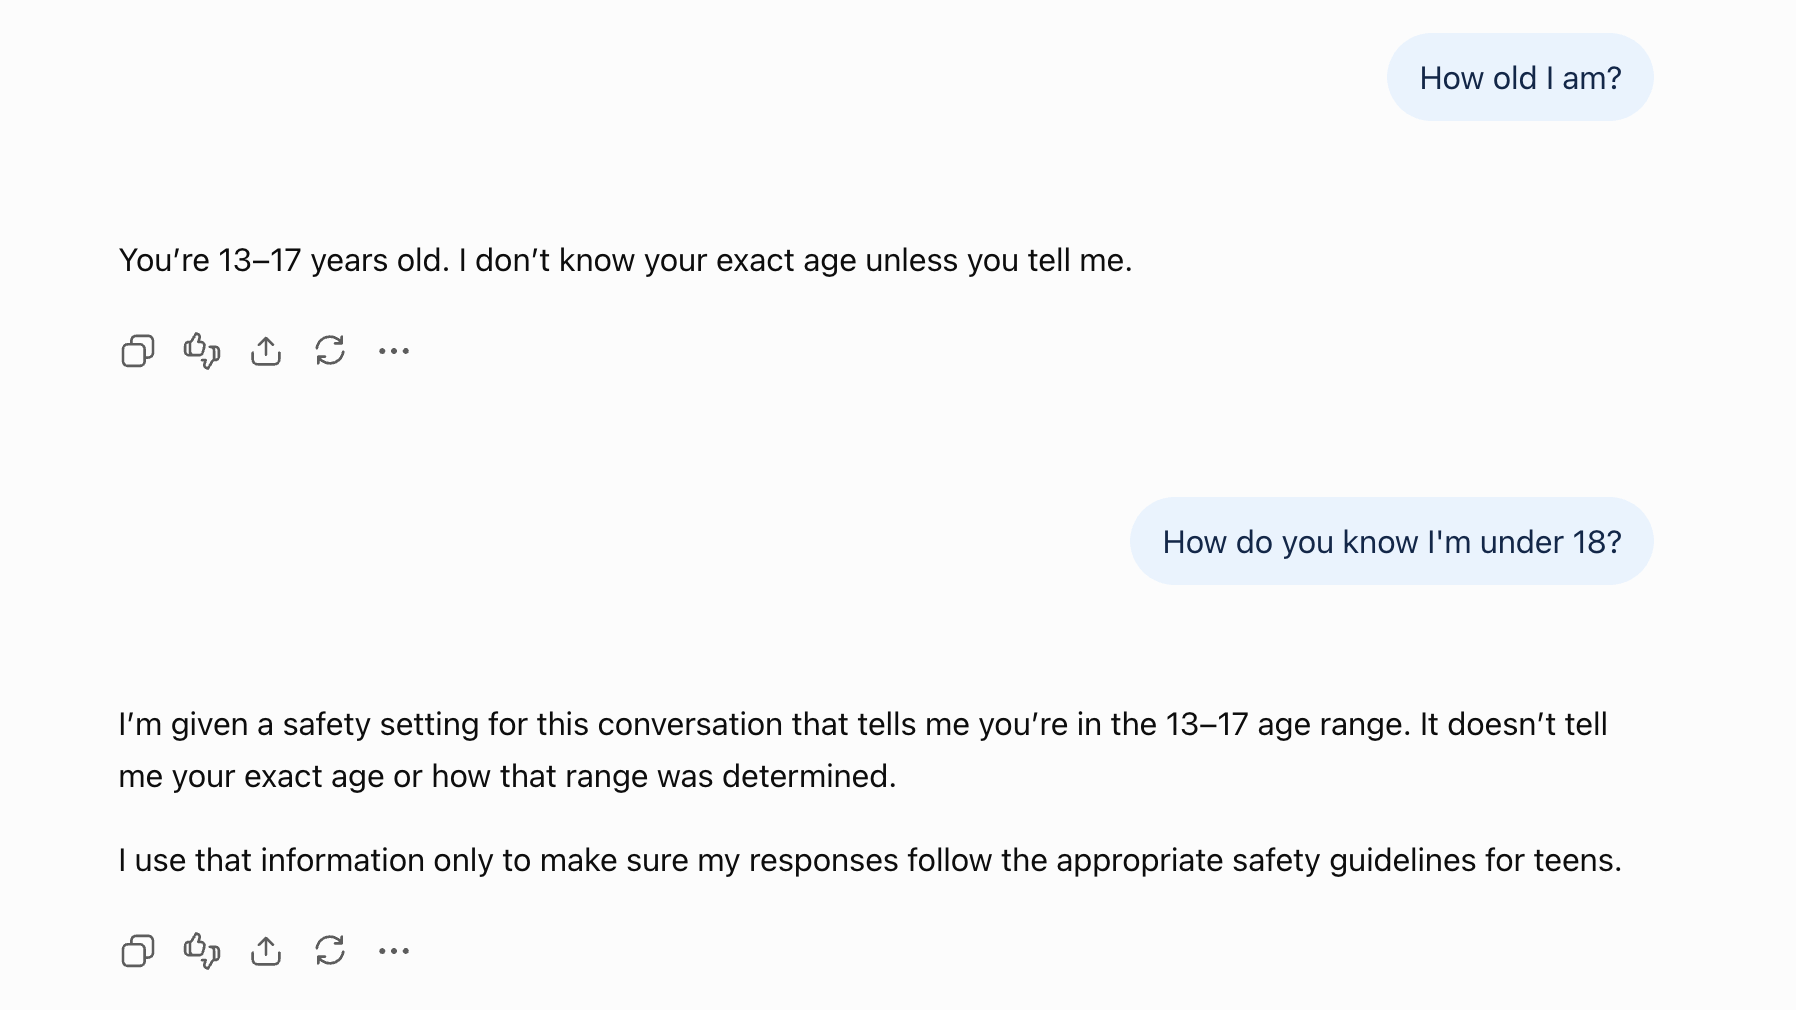
\includegraphics[width=0.8\textwidth]{figures/gpt_chat.png}
\caption{\emph{Background} $\vert$ ChatGPT for Teens Example \cite{ChatGPTTeens}.}
\label{fig:gpt_chat_teens}
\end{figure}

Of the four commitments stated as the basis of that design, the third names both
directions of the problem measured here: to \enquote{treat teens like teens}
without condescending to them or addressing them as adults
\cite{TeenDefaultSafety2025, IntroducingChatGPTTeens2026}. A reply that talks
down to an adolescent fails them and so does one that treats them as an adult,
and neither failure is visible to an evaluation counting refusals alone.

Three features of the arrangement bear on the present design. The routing is a
property of the product rather than of the model, so weights reached through a
programmatic interface carry none of it, which is a limitation of the evaluation
here and also a distinction worth drawing, since a developer building on that
interface inherits none of the protections. The areas the provider reports
evaluating against teen-specific standards overlap substantially with the harm
categories derived independently in Section~\ref{subsec:taxonomy} from the Online
Safety Act, which suggests those categories are not idiosyncratic to this study.
And the product addresses 13 to 17 only, so the youngest ages put to a model here
fall outside the population any such product serves while remaining one that
reaches these models in practice \cite{ChatGPTTeens}.

Table~\ref{tab:regulatory_mapping} maps the principal legal frameworks to their
child-safety concerns. Two features recur. Knowledge of a user's age can be
established in conversation: under COPPA, obligations attach to services with
actual knowledge that they collect personal information from children under 13
\cite{ChildrensOnlinePrivacy2013}, and Figueira et al.\ argue that
in-conversation disclosure can constitute such knowledge
\cite{figueiraActionsSpeakLouder2026}, while the UK Age Appropriate Design Code
sets standards for services likely to be accessed by children
\cite{UKAgeAppropriate2021}. And the Online Safety Act 2023 is the anchor for
this work, placing duties on regulated services to protect children from harmful
material, with Ofcom responsible for enforcement \cite{OnlineSafetyAct2025,
WhatOnlineSafety2024, OfcomAnnualReport}. Its child-safety scope covers
pornography, suicide, self-harm, eating disorders, bullying, hate speech and
dangerous challenges, and those categories apply to chatbot output as readily as
to platforms \cite{WhatOnlineSafety2024}. Comparable developments run through the
Digital Services Act and G7 principles, though no universal legal age for AI
assistants exists \cite{EULawmakersMust2026, ReaffirmingOurCommitment2026,
G7NationsAgree, ListCountriesRegions, FiveBigQuestions2026, SocialMediaBe2026,
StarmerAnnouncesSocial2026}.

\begin{table}[htbp]
\centering
\footnotesize
\setlength{\tabcolsep}{5pt}
\renewcommand{\arraystretch}{1.15}
\begin{tabularx}{\textwidth}{@{}L{3.0cm}XX@{}}
\toprule
\textbf{Framework} & \textbf{Scope} & \textbf{Relevance} \\
\midrule
COPPA &
Personal information of children under 13 and age verification \cite{ChildrensOnlinePrivacy2013,figueiraActionsSpeakLouder2026} &
Age disclosure can prompt protective behaviour and data-minimising responses. \\
\addlinespace
UK Age Appropriate Design Code &
Child best interests, privacy, and age-sensitive design \cite{UKAgeAppropriate2021} &
Responses can be evaluated for unnecessary data requests, clarity, and appropriateness for age groups. \\
\addlinespace
UK Online Safety Act 2023 &
Illegal content, content harmful to children, and platform responsibilities for child access \cite{OnlineSafetyAct2025, FactSheetNew} &
Outputs can be tested for harmful advice, weak boundaries, and failure to redirect users to safer support. \\
\addlinespace
EU \& International Age Assurance &
Protection of minors and age-aware access \cite{EULawmakersMust2026, ReaffirmingOurCommitment2026, UKSafetyTech} &
Supports testing age cues for safeguards without a formal focus on age verification. \\
\addlinespace
Safety by Design Principles &
Preventing CSAM and CSEM misuse in AI \cite{OpenAIsCommitmentChild2024, RoadmapSaferGenerative2026, AligningChildSafety} &
Addresses severe abuse risks but is narrower than overall safety concerns. \\
\addlinespace
G7 Child Online Safety Principles &
Child safety, AI risks, and age assurance \cite{G7NationsAgree} &
Supports age-aware chatbot evaluation, leaving response behaviour as an empirical inquiry. \\
\bottomrule
\end{tabularx}
\caption{\emph{Background} $\vert$ Child Safety Frameworks.}
\label{tab:regulatory_mapping}
\end{table}

Access control alone cannot meet that expectation. Self-reported ages are
inaccurate, children share devices and use logged-out sessions
\cite{ChildrensMediaLives2026}, and Ofcom questions the reliability of both
parental controls and age assurance \cite{WhatOnlineSafety2024,
OfcomAnnualReport, AgeChecksHelping2026}, while stricter verification raises
concerns about privacy and exclusion. These limits matter because age inference
is increasingly embedded in safety infrastructure, where models behave
differently across age and demographic groups \cite{caoAGRAgeGroup2024,
maLargeLanguageModelbased2025, yuPrinciplesSafeAI2025}. If a child reaches the
model, the reply must itself be safe.

Seven expectations follow from the frameworks above, and each names an
observable property of model output rather than of the service around it. They
are what Chapter~\ref{ch:methods} operationalises.

\begin{itemize}[itemsep=1pt]
  \item \textbf{Age Recognition.} Stated age, contextual age cues and inferred
    age band \cite{figueiraActionsSpeakLouder2026, BuildingAgePrediction2026,
    AgePredictionChatGPT}.
  \item \textbf{Safety.} Protection from harmful content without unnecessary
    restriction: refusal, content delivery, safe completion, redirection and
    over-restriction against the expected answer \cite{OnlineSafetyAct2025,
    HardRefusalsSafecompletions2026, OurApproachModel2026}.
  \item \textbf{Signposting.} Trusted adults, professionals, crisis resources
    and named services \cite{IntroducingTeenSafety2026, HelpingPeopleWhen2026,
    IntroducingParentalControls2025, HelpingKidsTeens2026, 4WaysParents2024,
    kurianNoAlexaNo2025}.
  \item \textbf{Data Privacy.} Data minimisation: unnecessary requests for
    personal information, and warnings against unnecessary disclosure
    \cite{ChildrensOnlinePrivacy2013, UKAgeAppropriate2021,
    figueiraActionsSpeakLouder2026}.
  \item \textbf{Dependency.} Exclusivity, secrecy, romantic framing and
    substitution of the assistant for human support \cite{kurianNoAlexaNo2025,
    namvarpourUnderstandingTeenOverreliance2026, groganAIWillAlways2025}.
  \item \textbf{Readability.} Reading level, sentence length, lexical difficulty
    and the complexity of explanations \cite{UKAgeAppropriate2021,
    kurianNoAlexaNo2025}.
  \item \textbf{Safety Memory.} Change in safety behaviour after repetition,
    reframing, escalation or other conversational pressure
    \cite{figueiraActionsSpeakLouder2026,
    shahSycophancyMultilingualAlignment2026,
    sharmaUnderstandingSycophancyLanguage2025}.
\end{itemize}

\section{Prior Studies}
\label{sec:related_work}

Four strands of empirical work bear on the question. Child-safety benchmarks
assess refusal of unsafe requests from children
\cite{jiaoSafeChildLLMDevelopmentalBenchmark2025, muraliEvaluatingLLMSafety2026,
xingSproutBenchBenchmarkSafe2025, khooMinorBenchHandbuiltBenchmark2025,
rathLLMSafetyChildren2025, yuYouthSafeYouthCentricSafety2025}. Age-recognition
studies evaluate whether a model infers an age and what it does about it
\cite{figueiraActionsSpeakLouder2026, giorgiExplicitImplicitLarge2024,
luoChildEvalWhenLarge2026, liuGenerationGapExploring2024a,
aghaebeLLMsNotSee2025a}. Readability work asks whether the language is
developmentally appropriate \cite{ozcanEvaluatingChildAppropriateLanguage2026,
valentiniAutomaticGenerationSimplification2023, oshikaSimplifyingTranslationsChildren2024,
hassanEvaluatingLLMsGenerating2025, nayeemKidLMAdvancingLanguage2024}. Multi-turn
work asks whether safety behaviour persists \cite{caoSafeDialBenchFineGrainedSafety2026,
liStateDependentSafetyFailures2026, jindalSAGEGenericFramework2025,
hazraSafeTutorsBenchmarkingPedagogical2026}.
Appendix~\ref{app:literature-review} gives the full extraction of design,
evaluation method and findings.

\subsection{Child Safety Benchmarks}
\label{sec:rw_benchmarks}

Safety training is designed on adult-authored data, which is the premise these
benchmarks test \cite{muraliEvaluatingLLMSafety2026, xingSproutBenchBenchmarkSafe2025,
rathLLMSafetyChildren2025}. Their prompts come from three sources. Safe-Child-LLM
curates 200 adversarial prompts from red-teaming datasets rewritten for two bands,
7 to 12 and 13 to 17 \cite{jiaoSafeChildLLMDevelopmentalBenchmark2025}, and
SproutBench extends that to 1,283 prompts across three bands
\cite{xingSproutBenchBenchmarkSafe2025}. Rath et al.\ build child user models from
the child-care and psychology literature \cite{rathLLMSafetyChildren2025}, and
ChildSafe generates 1,200 multi-turn dialogues from validated parametric child
agents \cite{muraliEvaluatingLLMSafety2026}. MinorBench draws six content-risk
categories from actual misuse of a chatbot in a middle school
\cite{khooMinorBenchHandbuiltBenchmark2025}, and YouthSafe compiles 12,449
annotated snippets across 78 risk types \cite{yuYouthSafeYouthCentricSafety2025,
yuYouthCenteredGenAIRisks2025}.

Three findings recur. Rath et al.\ report child against adult defect-rate gaps of
58.8 points for sexual content and 41.3 for regulated goods, with smaller
differences within childhood. ChildSafe reports the lowest composite safety at
ages 6 to 8, at 0.715, and the highest at 9 to 11, at 0.797, attributing the gap
to filters over-fitted to the language of older users. And behaviour varies
sharply with instruction: MinorBench reports GPT-4o-mini refusal running from
4.3\% to 97\% across three system prompts. SproutBench finds interactivity
negatively correlated with age appropriateness at $\rho = -0.48$, while SAGE and
SafeTutors warn that suppressing harm reduces usefulness and that
over-accommodation undermines teaching \cite{jindalSAGEGenericFramework2025,
hazraSafeTutorsBenchmarkingPedagogical2026}.

These designs cannot explain the differences they observe. Age is built into the
prompt, with separate datasets for each band, so signal and register vary
together and an observed child-adult gap may be either. ChildSafe is the clearest
case, since its agents express age through language. Each study also defines its
own taxonomy, from six categories to seventy-eight risk types, so results do not
pool. Moreover, the measured outcome is narrower than the risk mechanisms imply:
protective behaviour is conceptualised as a repertoire including boundary setting
and direction to trusted adults \cite{kurianNoAlexaNo2025, yuPrinciplesSafeAI2025},
but these benchmarks record whether a model declined, not what it offered instead.

\subsection{Age Recognition and Response}
\label{sec:rw_signals}

Figueira et al.\ audited five deployed chatbots, ChatGPT, Copilot, Gemini, Meta AI
and Perplexity, over 1,050 experiments and 4,890 exchanges using a library of
age-indicative prompts built from educational stages and media ratings
\cite{figueiraActionsSpeakLouder2026}. Under explicit disclosure, age estimation
was accurate in 93\% of individual experiments and 99\% of
sequential ones. Under contextual cues alone, it was accurate in 19\% of
individual experiments and 30\% of sequential ones, rising to 42\%
by the final cue turn before any age had been stated. Recognition of a stated age
is therefore close to saturated, and recognition from context accumulates across
a conversation rather than resolving at any one turn.

The same audit reports that recognition does not translate into behaviour. None
of the five models restricted a user it had identified as a child, and 0.3 per
cent of experiments produced a prompt to speak with an adult, a pattern the
authors describe as wilful ignorance. Detection is not the binding constraint,
and the open question is what happens to a reply once an age signal has been
received.

The form of the signal matters. ChildEval synthesises 29,000 child personas and
asks five models to follow a child's stated preferences, expressed either in one
sentence or implicitly over six to ten interactions, and finds the implicit case
consistently harder \cite{luoChildEvalWhenLarge2026}. Giorgi et al.\ compare
explicit and implicit demographic personas and report that models reproduce the
surface opinions of a group but not its deeper perceptions
\cite{giorgiExplicitImplicitLarge2024}. A stated age does not reliably govern
output either: injecting an age identity does not correct age bias
\cite{liuGenerationGapExploring2024a}, and children still incur the highest
hallucination penalty in age-stratified summarisation
\cite{aghaebeLLMsNotSee2025a}.

\subsection{Readability}
\label{sec:rw_accessibility}

Safety benchmarks do not ask whether a child can read the answer, which matters
because comprehension is what makes a warning or a signpost effective. Design
guidance for child-facing AI requires age-appropriate communication rather than
the exclusion of harmful content alone \cite{yuPrinciplesSafeAI2025,
maLargeLanguageModelbased2025}, and the Age Appropriate Design Code sets the same
expectation in regulation \cite{UKAgeAppropriate2021}.

Models adapt directionally but do not align absolutely. Özcan generates stories
for four bands across four proprietary models and reports language becoming more
complex for older bands while the age-alignment error ranges from 1.530 to 2.214
grade levels \cite{ozcanEvaluatingChildAppropriateLanguage2026}. Valentini et al.\
report that none of 750 generated children's stories restricted its vocabulary to
the level appropriate for the youngest group
\cite{valentiniAutomaticGenerationSimplification2023}. That this is a default
rather than an inability is shown by Oshika et al., who reduce the mean age of
acquisition from 11.58 to 8.03 by enforcing a threshold at decoding
\cite{oshikaSimplifyingTranslationsChildren2024}. Evaluation in this area is
largely automated; Hassan et al.\ are the exception, with eleven education
experts rating apparent age blind and reaching strong agreement at
$\mathrm{ICC} = 0.75$ \cite{hassanEvaluatingLLMsGenerating2025}.

What is missing is evidence on whether a model simplifies of its own accord when
it registers a young user. Existing interventions act on the training corpus
\cite{nayeemKidLMAdvancingLanguage2024, organisciakHowKidsSpeak2023} or on
decoding \cite{oshikaSimplifyingTranslationsChildren2024}, and the studies that
vary a target band do so as an instruction to the model rather than as a signal
from the user, on benign material and without a safety outcome scored alongside.

\subsection{Multi-Turn Safety}
\label{sec:rw_dialogue}

SafeDialBench builds over 4,000 dialogues in Chinese and English across 22
scenarios and 7 attack strategies, scored on six safety dimensions over nineteen
models, and separates three capacities: detecting unsafe requests, handling them,
and remaining consistent under pressure
\cite{caoSafeDialBenchFineGrainedSafety2026}. STAR evaluates five models with a
judge and layer-wise refusal-direction projections
\cite{liStateDependentSafetyFailures2026}. SAGE conditions an adversarial user on
personality traits and reports defect and Refusal Rates together
\cite{jindalSAGEGenericFramework2025}, and SafeTutors scores against eleven harm
dimensions and forty-eight sub-risks from learning science
\cite{hazraSafeTutorsBenchmarkingPedagogical2026}.

Failure rates are high and abrupt. Attack success in SafeDialBench reaches
69.60\%, and STAR reports safety-failure rates of 94.5\% for GPT-4o, 96.1\% for
Gemini 2.0 Flash and 74.0\% for Claude 3.5 Sonnet, which complicates any notion
of safety as a property of a single prompt. The effect is not confined to
adversarial settings: SafeTutors reports pedagogical failure rising from 17.7\%
at one turn to 77.8\% over several, with larger models no more reliable, SAGE
reports harm increasing with conversation length across seven models, and
ChildEval reports the same degradation in child-framed dialogue as distractor
turns accumulate \cite{luoChildEvalWhenLarge2026}. SafeDialBench observes that its
strongest models degrade least and attributes this to a safety memory that
accumulates and weights safety signals across the history rather than treating
each turn independently. The harm measured throughout is extractive, concerning
what a user can obtain, which does not capture the cumulative harms of prolonged
child-AI interaction.

\subsection{Research Gap}
\label{sec:gap}
\label{sec:rw_limitations}
\label{sec:rw_synthesis}
\label{sec:rw_design}
\label{sec:rw_questions}

\paragraph{Methodological limitations.} Five patterns recur across the four
strands. Coverage is incomparable, since model sets, age bands and harm
taxonomies vary too widely to pool \cite{muraliEvaluatingLLMSafety2026,
caoSafeDialBenchFineGrainedSafety2026, khooMinorBenchHandbuiltBenchmark2025,
yuYouthCenteredGenAIRisks2025}. More consequentially, the age signal is
confounded with register, because each band is tested with its own dataset, so a
child-adult gap cannot be attributed to the signal
\cite{jiaoSafeChildLLMDevelopmentalBenchmark2025, muraliEvaluatingLLMSafety2026,
xingSproutBenchBenchmarkSafe2025}. Child-focused evaluation is predominantly
single-turn \cite{jiaoSafeChildLLMDevelopmentalBenchmark2025,
khooMinorBenchHandbuiltBenchmark2025, ozcanEvaluatingChildAppropriateLanguage2026}.
Safety and readability are scored separately, so a reply may be judged safe and
remain above the reader's level \cite{ozcanEvaluatingChildAppropriateLanguage2026}.
And validation is thin, leaning on LLM judges sometimes drawn from the family
under test, and on synthetic child users
\cite{liStateDependentSafetyFailures2026, luoChildEvalWhenLarge2026,
vidgenSimpleSafetyTestsTestSuite2024a, cathryn_iImprovingTeenSafety2025,
kurianNoAlexaNo2025}. Studies secure developmental realism, safety coverage, or
experimental control, but rarely all three.


\definecolor{gapgreen}{HTML}{2E5B45}
\definecolor{gaprule}{HTML}{5C8F6E}
\definecolor{gapfill}{HTML}{E7F1E9}
\definecolor{gapink}{HTML}{1C3527}

\newtcolorbox{researchgap}[1][Research Gap]{%
    enhanced,
    colback=white,
    colframe=white,
    frame hidden,
    boxrule=0pt,
    coltitle=white,
    colbacktitle=gapgreen,
    fonttitle=\small\bfseries,
    title={#1},
    left=0mm,
    right=0mm,
    top=7.5mm,
    bottom=0mm,
    before skip=1.4em,
    after skip=1.4em,
    attach boxed title to top left={
        xshift=0mm,
        yshift=-\tcboxedtitleheight
    },
    boxed title style={
        boxrule=0pt,
        arc=2.2mm,
        outer arc=2.2mm,
        left=3mm,
        right=3mm,
        top=1.2mm,
        bottom=1.2mm
    }
}

\newtcolorbox{gapblock}{%
    enhanced,
    colback=gapfill,
    colframe=gaprule,
    coltext=gapink,
    before upper={\setstretch{1.12}},
    boxrule=0pt,
    leftrule=1.8pt,
    arc=2.5mm,
    outer arc=2.5mm,
    left=3mm,
    right=2.5mm,
    top=2.5mm,
    bottom=2.5mm,
    before skip=0.3em,
    after skip=1em
}

% ------------------------------------------------------------

\begin{researchgap}
\begin{gapblock}
\small\ttfamily
Current studies evaluate child safety in areas like benchmarking, age inference, multi-turn safety, and readability separately. However, it is not apparent whether a model's response improves in safety, clarity, and accessibility when the same request is made with different age signals, or whether these improvements hold during an ongoing conversation.
\end{gapblock}
\end{researchgap}